
\item A meter bridge is set-up as shown, to determine an unknown resistance `X' using a standard 10 ohm resistor. The galvanometer shows null point when tapping-key is at 52 cm mark. The end-corrections are 1 cm and 2 cm respectively for the ends A and B. The determined value of `X' is
    \begin{center}
        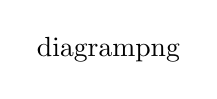
\begin{tikzpicture}
            \node at (0, 0) {diagrampng};
        \end{tikzpicture}
    \end{center}
    \begin{tasks}(2)
        \task 10.2 ohm
        \task 10.6 ohm
        \task 10.8 ohm
        \task 11.1 ohm
    \end{tasks}
